\section{Applications}
\label{sec:apps}

Before starting the description of the different categories of systems, I will give an overview of stream-based
applications. Traditionally stream processing has been applied to application domains requiring with very low tolerance
of failure. These applications are able to produce meaningful results only when the processing is carried out without
any loss of data or approximation.

Financial algorithmic trading~\cite{streambase-algo} is an example of such an application. Investment banks, trading on the stock market need
to process a great deal of financial events in real-time. Complex algorithms are used to capture the current situation
of the market and give hints on profitable trades exploiting temporary arbitrage conditions. For these applications the
focus is on efficiency: being able to make a trade even a split second before a competitor is the key to achieve maximum
profits. In this scope the necessity of processing all the available information is evident, as a wrong choice based on
approximate data could mean the loss of large amounts of money.

On the other hand, there are some classes of applications which are able to operate correctly even not all the data can
be correctly process~\cite{phi}. In many cases a certain degree of failure in the system is tolerable and does not hinder the application from producing
meaningful results. In particular I am going to focus on two categories of applications which are capable of producing meaningful
results under partial failure: environmental sensing and Internet monitoring. 

\subsection{Environmental Monitoring}
\label{envmon}

The first domain of applications I will take into consideration is large-scale scientific sensing, in
particular I will describe projects dealing with large-scale environmental monitoring.  In recent years,
the availability of cheap micro-sensing technology has unleashed the capability of sensing at an
unprecedented scale. We can expect in the future to see everything of material significance being
"sensor-tagged" and report its state or location in
real-time~\cite{irisnet,qpsn,stream-processing-challanges}. At the present time, great number of
large-scale sensing projects are being developed and we can expect even more to come into
place~\cite{earthscope,neon,casa-lead,swissexp}.

One area in which large scale sensing has flourished is environmental monitoring. The growing concern
about climate change has brought a lot of attention to environmental studies, and many large-scale
sensing projects have been launched to better understand the behaviour of many natural processes.
Examples of such efforts are for instance the Earthscope~\cite{earthscope} and the Neon~\cite{neon}
projects.

Earthscope is a multi-disciplinary project across earth sciences to study the geophysical structure and
evolution of the American continent. It uses a large number of sensors geographically distributed over
the whole continent to answer some of the outstanding questions in Earth Sciences by looking deeper, at
increased resolution, and integrating diverse measurements and observations. Thousands of geophysical
instruments measure the motion of Earth's surface, record seismic waves and recover rock samples from
depths at which earthquakes originate. All the collected data is freely available and a large community
of scientists is conducting several multidisciplinary researches based on it. Examples of sensing
projects within Earthscope include the constant monitoring of the San Andreas fault, and the Plate Bound
Observatory, which collects information about the tectonic movements across the active boundary zone
between the Pacific and North American plates in the western United States.

NEON stands for national ecological observation network. This project aims at creating a new national
observatory network to collect ecological and climatic observations across the United States. It is an
example of continental-scale research platform for discovering and understanding the impacts of climate
change, land-use change, and invasive species on ecology. It is the first observatory designed to detect
and enable forecasting of ecological change at continental scales over multiple decades. Obtaining this
kind of data over a \mbox{long-term} period is crucial to improving ecological forecast models and will
greatly help the understanding the effects of human interference on climate change.  These are just two
examples of large-scale monitoring projects, and many others already exists or will be started in the
near future~\cite{testban,skysurvey,neon,usvo}. 

Environmental sensing is a natural application for stream processing. A constant flow of measurements is
generated by a large number of sensors, stream processing systems offer an intuitive and flexible
paradigm to harness the complexity of mining such a high volume of data. It also give the possibility of
obtaining real-time picture of the measured phenomena, enabling quick reactions to possibly disruptive
events. The core components of these projects are sensing stations geographically widely distributed and
often subject to harsh conditions. In this scenario, the failure of these sensing devices is not going to
be uncommon and often their replacement is going to be problematic. Long running continuous queries need
to be able to deal with some missing data, adapting to the new conditions and reporting the achieved
quality of service. To collect and process all the data at all times is most probably infeasible and it
is important for the computing backbone of such projects to be able to withstand a certain degree of
failure within the system~\cite{dependable-is-sensing}.

I will now present two more specific examples of infrastructures aiming at supporting large-scale sensing
projects.  The first is concerned with meso-scale weather monitoring, while the second focuses on the
collection of data from environmental sensors in a more general purpose fashion. Both project could take
advantage from my research, by enabling them to produce results in real-time and to better operate in the
occurrence of failure at the sources or computing nodes.

\textbf{Distributed Collaborative Adaptive Sensing} Meso-scale weather events, such as tornadoes and
hurricanes, cause every year a large number of deaths and a great deal of damage to infrastructures.
Being able to understand and predict when these hazardous weather conditions will occur is going to
greatly mitigate their consequences.

In this regard, the National Science Foundation has recently established the center for
\textit{Collaborative Adaptive Sensing of the Atmosphere (CASA)}~\cite{casa}. This project aims at
enhancing the current infrastructure of long-range weather observing radars, with a large number of small
solid-state radars able to increase the sampling resolution throughout the entire troposphere. Although
current \mbox{long-range} radar technology allows the coverage of large areas with a relative small
number of devices, these are not able to correctly measure the lowest part of the atmosphere in areas
faraway from the radar. This is due to Earth curvature and terrain-induced blockage.  This new sensing
paradigm, based on a greater number of smaller devices, goes under the name of Distributed Collaborative
Adaptive Sensing (DCAS). Distributed refers to the use of numerous small and inexpensive radars, spread
near enough to fully measure the area even at lower altitudes where the traditional approach fails.
Collaborative refers to the coordination of multiple devices covering overlapping areas to increase the
resolution and the precision of the measurements compared to a single radar. Adaptive refers to the
ability of the infrastructure to dynamically adjust its configuration based on the current weather
conditions and user needs.

Another project, closely linked to CASA is the \emph{Linked Environments for Atmospheric Discovery
(LEAD)}~\cite{lead}. This gives scientists the tools with which they can automatically spawn weather
forecast models in response to real-time weather events for a desired region of interest. It is a
middleware that facilitates the adaptive utilization of distributed resources, sensors and workflows.
While CASA is primarily concerned with the reliable collection of the data, LEAD is the backbone
processing infrastructure. It allows the automation of time consuming and complicated tasks associated
with meteorological science through the creation of workflows. The "workflow" tool links data management,
assimilation, forecasting, and verification applications into a single experiment. Weather information is
available to users in real-time, whom are not being restricted to pre-generated data, greatly expanding
their experimental opportunities.

The integration of these two systems offers an invaluable infrastructure to atmospheric scientists
\cite{casa-lead}.  First of all, it allows meteorologists to directly interact with data from the
instruments as well as control the instruments themselves. Also, unlike traditional forecasting
approaches, it allows the establishment of interactive closed loops between the forecast analysis and the
instruments. This sensing paradigm based on numerous input devices and the possibility of processing
their data into a forecasting model is changing the way meso-scale weather events are detected and will
help to greatly mitigate their impact. Stream processing has the potential of enhancing the CASA/LEAD
infrastructure, extending its real-time monitoring capabilities. In this infrastructure, when implemented
at larger scale, failure is going to be the common case. CASA is built from small weather stations, and
it is designed to withstand failure at the sources and to reconfigure at run-time~\cite{casa}. This means
that during long running queries, the backbone processing system is likely to be affected by failure at
the sources and experience variations in the quality of the results.  For these reasons, this scenario
would be a prefect test-bed onto which exploring ways to operate a large-scale monitoring system under
constant partial failure, while constantly measuring the achieved quality of processing.

% \paragraph{The Swiss Experiment} Another example of large-scale environmental sensing project is
% represented by the Swiss Experiment~\cite{swissexp}. The aim of the project is to enable effective
% real-time environmental monitoring through wireless sensor networks and a modern, generic
% cyber-infrastructure. It is a collaborative projects with many contributions on different scientific
% and technological aspects.
%  Within the scope of the project, a new wireless sensor network technology has been developed, called
% SensorScope~\cite{sensorscope}. This is an out-of-the-box environmental monitoring infrastructure based
% on inexpensive wireless sensor nodes. SensorScope is both a hardware and software architecture. It
% falls into the category of time-driven networks, as the stations intermittently transmit environmental
% data to a sink, which in turn make the received data available through a number of interfaces. It has
% been deployed and tested in many occasions, being one of the fundamental building block employed in the
% project. It was used to monitor the quality of the water in the Le Boiron de Morges river, on Le Genepi
% rock glacier, to monitor dangerous mud streams, and on the Grand St.  Bernard pass, to obtain a very
% precise map of evaporation of the area.
%  PermaSense~\cite{permasense} is another technological effort within the project. It aims at the
% development of an innovative sensor infrastructure for automated, unattended long-term data acquisition
% in the extremes of high-alpine regions. The goal is to investigates the effect of permafrost in
% high-alpine environments.
%  All the data gathered by the project is made available through a number of interfaces like GoogleMaps
% and SenseMap~\cite{sensemap}. The acquisition and storage of the data is also performed in different
% ways. It is saved in a wiki, in comma separated values files, even though the most interesting way is
% through the GSN (Global Sensor Networks).  This is a database software middleware designed to
% facilitate the deployment and programming of sensor networks. Large-scale, long-running monitoring
% tasks like the ones in the aims of the Swiss Experiment are likely to experience failure, either at the
% sources and in the distributed backbone processing infrastructure. GSN, the tool employed for
% \mbox{real-time} data mining within this project, reacts to failure by simply releasing the associated
% resources and continuing the processing without them~\cite{gsn-book}. This behaviour could be improved,
% by introducing the ability of introducing quality-awareness in its processing. Extending GSN in this
% regard, would allow it to better operate in hostile environments characterized by a high occurrence of
% failure. This would enhance its capabilities, providing users with a better understanding of
% approximate results and the behaviour of the system.


% \begin{figure}[b!] \centering 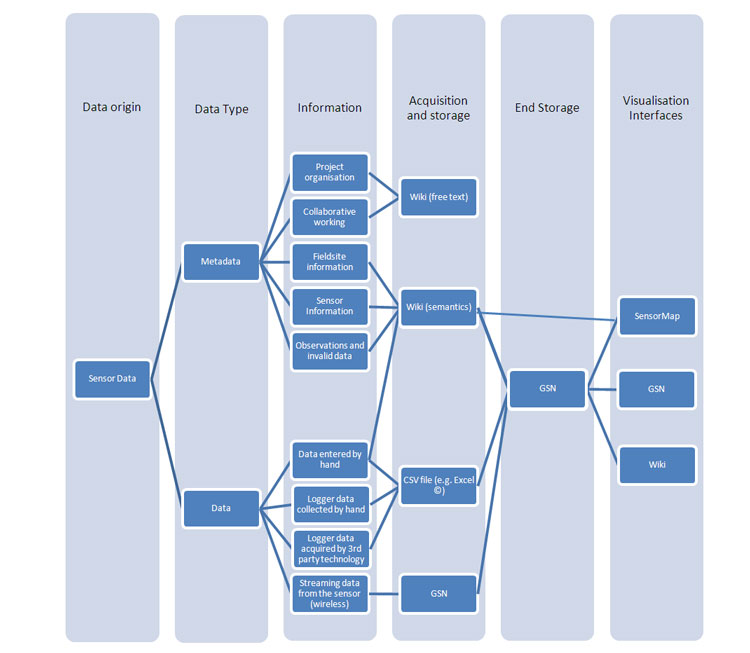
\includegraphics[scale=0.4]{img/swissex-overview.jpg} \label{img:swissex}
% \caption{Outline of the SwissEx infrastructure} \end{figure}


% \subsubsection*{Astrophysics} 
\label{sec:astro} 
%\notemf{I find the structure here to be a little confusing. Some options: a) eliminate astrophysics b) talk of swiss
%experiment in the introduction of the paragraph, as it is a more general purpose experiment c) leave it like this d)
%your say?}

\begin{structure}
	\item Application of StreamGlobe, explained in Section \ref{sec:streamglobe}
\end{structure}

StarGlobe: Grid-Based Data Stream Processing in e-Science \cite{starglobe-grid}


\subsection{Environmental Monitoring}
\label{envmon}

The first domain of applications I will take into consideration is large-scale scientific sensing, in
particular I will describe projects dealing with large-scale environmental monitoring.  In recent years,
the availability of cheap micro-sensing technology has unleashed the capability of sensing at an
unprecedented scale. We can expect in the future to see everything of material significance being
"sensor-tagged" and report its state or location in
real-time~\cite{irisnet,qpsn,stream-processing-challanges}. At the present time, great number of
large-scale sensing projects are being developed and we can expect even more to come into
place~\cite{earthscope,neon,casa-lead,swissexp}.

One area in which large scale sensing has flourished is environmental monitoring. The growing concern
about climate change has brought a lot of attention to environmental studies, and many large-scale
sensing projects have been launched to better understand the behaviour of many natural processes.
Examples of such efforts are for instance the Earthscope~\cite{earthscope} and the Neon~\cite{neon}
projects.

Earthscope is a multi-disciplinary project across earth sciences to study the geophysical structure and
evolution of the American continent. It uses a large number of sensors geographically distributed over
the whole continent to answer some of the outstanding questions in Earth Sciences by looking deeper, at
increased resolution, and integrating diverse measurements and observations. Thousands of geophysical
instruments measure the motion of Earth's surface, record seismic waves and recover rock samples from
depths at which earthquakes originate. All the collected data is freely available and a large community
of scientists is conducting several multidisciplinary researches based on it. Examples of sensing
projects within Earthscope include the constant monitoring of the San Andreas fault, and the Plate Bound
Observatory, which collects information about the tectonic movements across the active boundary zone
between the Pacific and North American plates in the western United States.

NEON stands for national ecological observation network. This project aims at creating a new national
observatory network to collect ecological and climatic observations across the United States. It is an
example of continental-scale research platform for discovering and understanding the impacts of climate
change, land-use change, and invasive species on ecology. It is the first observatory designed to detect
and enable forecasting of ecological change at continental scales over multiple decades. Obtaining this
kind of data over a \mbox{long-term} period is crucial to improving ecological forecast models and will
greatly help the understanding the effects of human interference on climate change.  These are just two
examples of large-scale monitoring projects, and many others already exists or will be started in the
near future~\cite{testban,skysurvey,neon,usvo}.

Environmental sensing is a natural application for stream processing. A constant flow of measurements is
generated by a large number of sensors, stream processing systems offer an intuitive and flexible
paradigm to harness the complexity of mining such a high volume of data. It also give the possibility of
obtaining real-time picture of the measured phenomena, enabling quick reactions to possibly disruptive
events. The core components of these projects are sensing stations geographically widely distributed and
often subject to harsh conditions. In this scenario, the failure of these sensing devices is not going to
be uncommon and often their replacement is going to be problematic. Long running continuous queries need
to be able to deal with some missing data, adapting to the new conditions and reporting the achieved
quality of service. To collect and process all the data at all times is most probably infeasible and it
is important for the computing backbone of such projects to be able to withstand a certain degree of
failure within the system~\cite{dependable-is-sensing}.

I will now present two more specific examples of infrastructures aiming at supporting large-scale sensing
projects.  The first is concerned with meso-scale weather monitoring, while the second focuses on the
collection of data from environmental sensors in a more general purpose fashion. Both project could take
advantage from my research, by enabling them to produce results in real-time and to better operate in the
occurrence of failure at the sources or computing nodes.

\textbf{Distributed Collaborative Adaptive Sensing} Meso-scale weather events, such as tornadoes and
hurricanes, cause every year a large number of deaths and a great deal of damage to infrastructures.
Being able to understand and predict when these hazardous weather conditions will occur is going to
greatly mitigate their consequences.

In this regard, the National Science Foundation has recently established the center for
\textit{Collaborative Adaptive Sensing of the Atmosphere (CASA)}~\cite{casa}. This project aims at
enhancing the current infrastructure of long-range weather observing radars, with a large number of small
solid-state radars able to increase the sampling resolution throughout the entire troposphere. Although
current \mbox{long-range} radar technology allows the coverage of large areas with a relative small
number of devices, these are not able to correctly measure the lowest part of the atmosphere in areas
faraway from the radar. This is due to Earth curvature and terrain-induced blockage.  This new sensing
paradigm, based on a greater number of smaller devices, goes under the name of Distributed Collaborative
Adaptive Sensing (DCAS). Distributed refers to the use of numerous small and inexpensive radars, spread
near enough to fully measure the area even at lower altitudes where the traditional approach fails.
Collaborative refers to the coordination of multiple devices covering overlapping areas to increase the
resolution and the precision of the measurements compared to a single radar. Adaptive refers to the
ability of the infrastructure to dynamically adjust its configuration based on the current weather
conditions and user needs.

Another project, closely linked to CASA is the \emph{Linked Environments for Atmospheric Discovery
(LEAD)}~\cite{lead}. This gives scientists the tools with which they can automatically spawn weather
forecast models in response to real-time weather events for a desired region of interest. It is a
middleware that facilitates the adaptive utilization of distributed resources, sensors and workflows.
While CASA is primarily concerned with the reliable collection of the data, LEAD is the backbone
processing infrastructure. It allows the automation of time consuming and complicated tasks associated
with meteorological science through the creation of workflows. The "workflow" tool links data management,
assimilation, forecasting, and verification applications into a single experiment. Weather information is
available to users in real-time, whom are not being restricted to pre-generated data, greatly expanding
their experimental opportunities.

The integration of these two systems offers an invaluable infrastructure to atmospheric scientists
\cite{casa-lead}.  First of all, it allows meteorologists to directly interact with data from the
instruments as well as control the instruments themselves. Also, unlike traditional forecasting
approaches, it allows the establishment of interactive closed loops between the forecast analysis and the
instruments. This sensing paradigm based on numerous input devices and the possibility of processing
their data into a forecasting model is changing the way meso-scale weather events are detected and will
help to greatly mitigate their impact. Stream processing has the potential of enhancing the CASA/LEAD
infrastructure, extending its real-time monitoring capabilities. In this infrastructure, when implemented
at larger scale, failure is going to be the common case. CASA is built from small weather stations, and
it is designed to withstand failure at the sources and to reconfigure at run-time~\cite{casa}. This means
that during long running queries, the backbone processing system is likely to be affected by failure at
the sources and experience variations in the quality of the results.  For these reasons, this scenario
would be a prefect test-bed onto which exploring ways to operate a large-scale monitoring system under
constant partial failure, while constantly measuring the achieved quality of processing.

% \paragraph{The Swiss Experiment} Another example of large-scale environmental sensing project is
% represented by the Swiss Experiment~\cite{swissexp}. The aim of the project is to enable effective
% real-time environmental monitoring through wireless sensor networks and a modern, generic
% cyber-infrastructure. It is a collaborative projects with many contributions on different scientific
% and technological aspects.
%  Within the scope of the project, a new wireless sensor network technology has been developed, called
% SensorScope~\cite{sensorscope}. This is an out-of-the-box environmental monitoring infrastructure based
% on inexpensive wireless sensor nodes. SensorScope is both a hardware and software architecture. It
% falls into the category of time-driven networks, as the stations intermittently transmit environmental
% data to a sink, which in turn make the received data available through a number of interfaces. It has
% been deployed and tested in many occasions, being one of the fundamental building block employed in the
% project. It was used to monitor the quality of the water in the Le Boiron de Morges river, on Le Genepi
% rock glacier, to monitor dangerous mud streams, and on the Grand St.  Bernard pass, to obtain a very
% precise map of evaporation of the area.
%  PermaSense~\cite{permasense} is another technological effort within the project. It aims at the
% development of an innovative sensor infrastructure for automated, unattended long-term data acquisition
% in the extremes of high-alpine regions. The goal is to investigates the effect of permafrost in
% high-alpine environments.
%  All the data gathered by the project is made available through a number of interfaces like GoogleMaps
% and SenseMap~\cite{sensemap}. The acquisition and storage of the data is also performed in different
% ways. It is saved in a wiki, in comma separated values files, even though the most interesting way is
% through the GSN (Global Sensor Networks).  This is a database software middleware designed to
% facilitate the deployment and programming of sensor networks. Large-scale, long-running monitoring
% tasks like the ones in the aims of the Swiss Experiment are likely to experience failure, either at the
% sources and in the distributed backbone processing infrastructure. GSN, the tool employed for
% \mbox{real-time} data mining within this project, reacts to failure by simply releasing the associated
% resources and continuing the processing without them~\cite{gsn-book}. This behaviour could be improved,
% by introducing the ability of introducing quality-awareness in its processing. Extending GSN in this
% regard, would allow it to better operate in hostile environments characterized by a high occurrence of
% failure. This would enhance its capabilities, providing users with a better understanding of
% approximate results and the behaviour of the system.


% \begin{figure}[b!] \centering 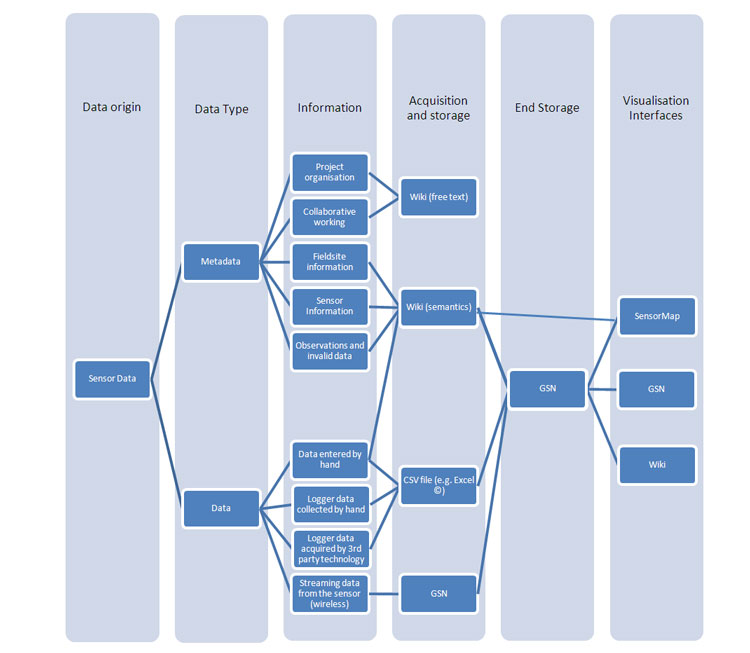
\includegraphics[scale=0.4]{img/swissex-overview.jpg} \label{img:swissex}
% \caption{Outline of the SwissEx infrastructure} \end{figure}


% \subsubsection*{Astrophysics} 
\label{sec:astro} 
%\notemf{I find the structure here to be a little confusing. Some options: a) eliminate astrophysics b) talk of swiss
%experiment in the introduction of the paragraph, as it is a more general purpose experiment c) leave it like this d)
%your say?}

\begin{structure}
	\item Application of StreamGlobe, explained in Section \ref{sec:streamglobe}
\end{structure}

StarGlobe: Grid-Based Data Stream Processing in e-Science \cite{starglobe-grid}



\subsection{Internet Monitoring}
\label{sec:phi}
The second class of stream-based applications, which can successfully operate under partial failure, is large-scale
Internet monitoring. In this case, the data streams are not produced by sensors in the physical world like in the case
of sensor networks. They measure instead, non physical quantities describing events happening within the global network
infrastructure. Internet security is perhaps the most important challenge facing computing today. The spread of malicious
software (viruses, worms, spyware and the like) is constantly growing~\cite{mcafee-report_2q2009}, and comes at a
serious cost for individual users as well as for businesses. 
The arousal of worldwide botnets seems unstoppable, with hundred of thousands of machines
infected everyday, and is a powerful tool to launch DDoS attacks and to spread the ever increasing amount of spam.
It is clear then, how vital it is to the future development of the Internet to be able to monitor the spread of infections,
and in general its overall "health" condition.

\subsubsection*{Public Health fot the Internet ($\varphi$)}
The authors of~\cite{phi} propose a new grand challenge to the computer science community called Public Health for the
Internet. PHI (or $\varphi$) has precisely this objective, to enable machines on the Internet to join forces to establish a
"community health watch" infrastructure that aggressively share, analyses and acts upon information observed at various
machines. The idea is to allow endpoint traffic observations to be shared across machines for the common good.
It is useful to consider the problem in terms of medical analogies. Medicine, as a discipline, is concerned with curing
individuals, and focuses less on widespread problems. The complementary field of Public Health, instead, deals with the
well being of the population as a whole. It is concern in identifying and mitigating the spread of a disease in a
population. So far, Internet security has been perceived in a way which resembles medicine, it has been focused on
individuals or small groups. Firewalls and anti-viruses, even though somehow effective, do not protect and monitor the
community as a whole. The $\varphi$ approach, instead, aims at monitoring the Internet at large, exploiting the information
collaboratively gathered by a large number of monitoring machines.

The idea of being able to monitor the Internet at large is not new. Previously it has been proposed to build a "Center
for Disease Control" for the Internet~\cite{own-the-internet}. The problem with this approach is basic: who runs the
center and who controls the controller? Also, a centralized approach would lack the scalability to be able to
effectively monitor the Internet as a whole. Instead, the $\varphi$ proposal is to establish a global collaborative
infrastructure, able to monitor the Internet at scale. This decentralized architecture very much resembles a
peer-to-peer system, being constituted by a number of independent and hierarchically equivalent monitoring entities.
The $\varphi$ architecture would be composed of at least three main components. First of all, a variety of network
"sensors" software modules, gathering information about the network security and performance at each endpoint. 
The second component would be a peer-to-peer protocol, allowing the dissemination of this information, in order to
enable collaborative analysys of it. Third, there is the need for easy to use, intuitive end-user software interfaces,
both to incent users to join the collective, and to encourage them to be more proactively aware of their online
security.

\paragraph{Stream Processing and \textbf{$\varphi$}}
A key component of the $\varphi$ challange involves distributed, real-time information management. This collectively
gathered security and performance measurements will take the form of distributed streams of data, coupled with
historical repositories. The streams will be generated by a variety of network "sensors", based on log events from
firewalls, operating systems and many other network applications. The amount of streams and produced data is going to be
massive and one of the challange for such a system is to be able to effectively process it. Also, because of the scale
at which the system is designed to operate, it is unfeasible to collect all the data at all times. In particular, since
this application focuses on detecting the spread of infections and attacks, it is very likely that many of the
compromised endpoints won't be able to correctly report their measurements. In fact, partial failure is going to be the
common operational mode for the system. Despite this, though, the infrastructure should be able to identify threats and
to react to them. Having stated these constraints, it is evident how distributed stream processing would be the correct
paradigm to tackle the problem. In particular, this application is ideal for our dependable stream processing system,
which is designed to be massively scalable and able to operate in presence of failure.



%Internet Telescopes \cite{internet-telescope}




%\subsection{Financial Data Processing}
\label{sec:finance}

Algorithmic Trading


\newpage
